\chapter{Implementation of the standard C descriptors for C-Fortran interoperability}\label{c:isocbinding}

Code hosted on \href{https://github.comhttps://github.com/}{\texttt{https://github.com/}}.

\noindent Sourcery Institute: \href{https://github.com/sourceryinstitute/}{\texttt{sourceryinstitute}}

\noindent\href{https://github.com/sourceryinstitute/iso_Fortran_binding/}{\texttt{iso\_fortran\_binding}}

\noindent\texttt{GCC}: \href{https://github.com/gcc-mirror/gcc/blob/master/libgfortran/}{\texttt{https://github.com/gcc-mirror/gcc/blob/master/libgfortran/}}

\noindent \texttt{GCC} definitions: \href{https://github.com/gcc-mirror/gcc/blob/master/libgfortran/ISO_Fortran_binding.h}{\texttt{ISO\_Fortran\_binding.h}}

\noindent\texttt{GCC} implementation: \href{https://github.com/gcc-mirror/gcc/blob/master/libgfortran/runtime/ISO_Fortran_binding.c}{\texttt{/runtime/ISO\_Fortran\_binding.c}}

The Fortran 2018 standard \cite{fortran} defines a standard set of C structures and functions that give C the ability to access and operate on Fortran variables and objects. The structures contain all the information needed to fully explore most Fortran objects from C programmes. The functions perform unit operations that can be used together to perform more complex ones. These structures and functions standardise and greatly expand current C-Fortran interoperability. This paper summarises their use and implementation.

\section{Introduction}

Fortran has historically been the de facto language of scientific computing. However, C-type languages such as C/C++ have gained much traction since the 90s due to their popularity in software development. Furthermore, the large degree of compatibility between C and higher level languages such as Python, Java, Objective-C and others have made C the center piece of general purpose computing.

The popularity of C-type languages has resulted in an increase of scientific computing codes written in them, particularly C++ and Python due to their ready-made data structures and algorithms. However, when it comes to high performance computing in numerical applications Fortran still has the edge. In order to get the best of both worlds however, increasing C-Fortran interoperability is of the utmost importance.

C-Fortran interoperability has existed in a rudimentary fashion since the Fortran 2003 standard \cite{fortran}. Compiler manufacturers are free to add non-standard compliant functionality which expand language features. These expansions are compiler-specific and limit code compatibility between different systems and compilers. Often, these compiler-specific additions are standardised and expanded by the standards committee in future releases.

The Fortran 2018 standard did so with the C-descriptors of Fortran variables as well as basic functions to query and utilise them. They expand and homogenise the capabilities of various compiler-specific expansions, increasing software portability and interoperability.

\section{C descriptor structure}

The C descriptors are C structures which act as non-generic containers for Fortran variables. The C descriptor structure contains various member variables that allow one to fully explore and use Fortran objects within C. The C descriptor structure makes use of a few custom types, among which is another structure \texttt{CFI\_dim\_t};
\begin{itemize}
    \item \texttt{CFI\_index\_t lower\_bound}: lower bound of the dimension being described;
    \item \texttt{CFI\_index\_t extent}: number of elements in the dimension being described;
    \item \texttt{CFI\_index\_t sm}: memory stride for the dimension, i.e. the difference in bytes between the addresses of successive elements in the dimension being described.
\end{itemize}
The actual structure of the C descriptor is as follows,
\begin{itemize}
    \item \texttt{void *base\_address}: pointer to the base address of the fortran object or first element of the array being described;
    \item \texttt{size\_t elem\_len}: storage size in bytes of the object or element of the array being described;
    \item \texttt{CFI\_rank\_t rank}: rank of the array described, rank 0 denotes a scalar;
    \item \texttt{CFI\_type\_t type}:  type of the object described, each interoperable type has a specific type identifier;
    \item \texttt{CFI\_attribute\_t attribute}: denotes whether the object is allocatable, pointer or nonallocatable nonpointer, each has a unique value;
    \item \texttt{CFI\_dim\_t dim}: dimensional information.
\end{itemize}

C is a weak, statically typed language; \emph{statically typed} means that types are checked at compile and runtime, \emph{weak} means they can be converted into other types via pointer casting. This is often the source of many a headache and bug, but can double as a poor-man's polymorphism\footnote{Polymorphism is when a variable or function, can be of different types.}. This is readily exploited by the functions which utilise the C descriptors. \Cref{f:cast} illustrates how C looses track of the full size of the structure, but since it knows the size of the \texttt{dim} structure as well as the rank of the object being described, one can fully traverse the object.
\begin{figure}
    \centering
    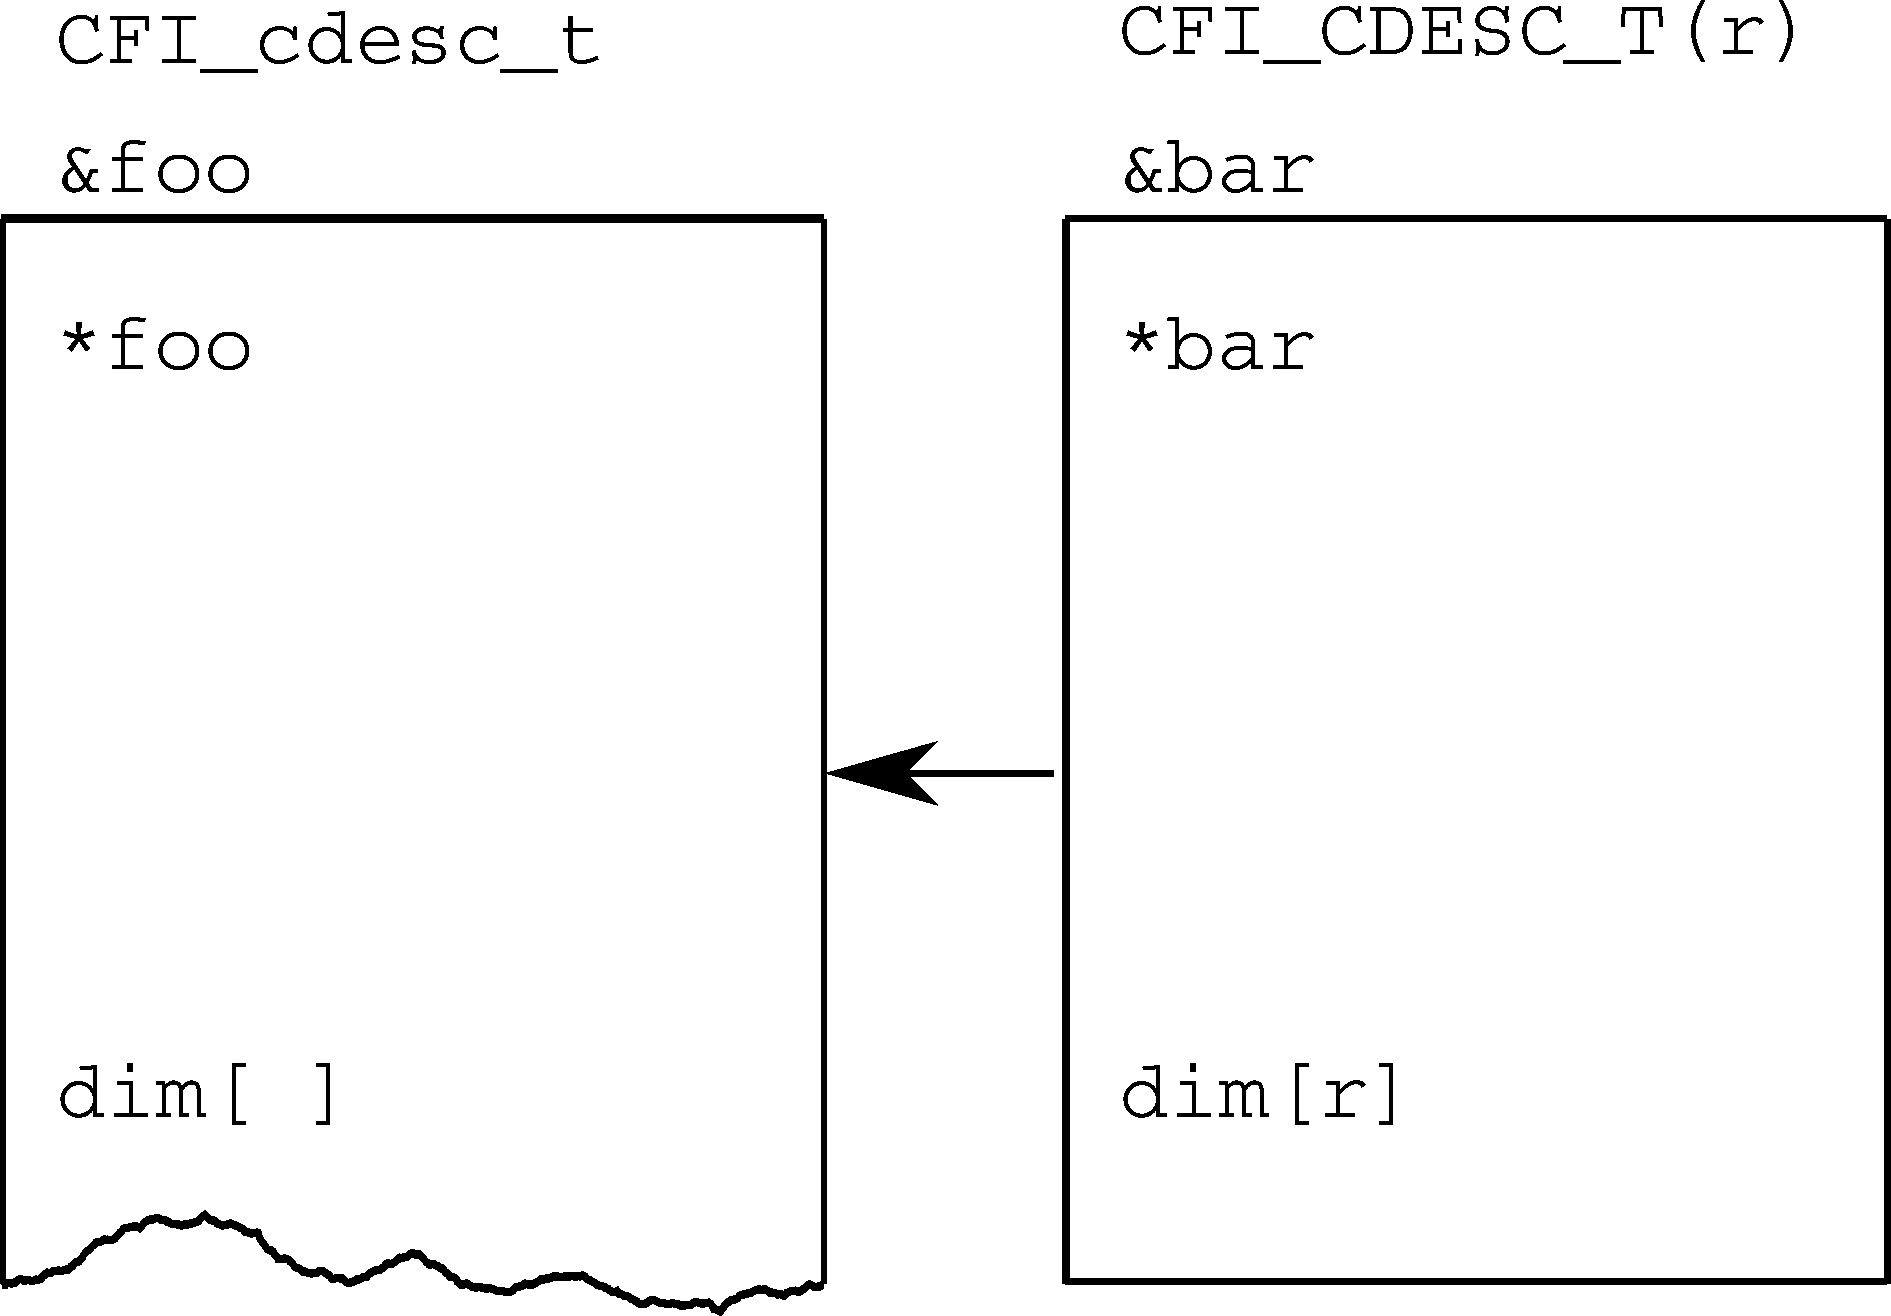
\includegraphics[width=0.5\linewidth]{cdesc.pdf}
    \caption[C descriptor with rank \texttt{r} being cast into one with unspecified rank.]{C descriptor with rank \texttt{r} being cast into one with unspecified rank. C looses track of exactly how large the object is, but given the value of the rank element \texttt{r}, the size of a single element of \texttt{dim} and the information contained within the \texttt{dim} member variables, the object can be fully explored.}
    \label{f:cast}
\end{figure}
As a result, developers are \emph{strongly} advised to use the standard functions and---if need be---create their own, more complex ones if they want to manipulate the C object.

\section{C descriptor functions}

As aforementioned, the functions defined by the standard \cite{fortran} allow the user to use and explore Fortran objects from within C;
\begin{itemize}
    \item \texttt{CFI\_establish}: updates the C descriptor variable to establish it as a variable that would allow the program to access fortran variables;
    \item \texttt{CFI\_address}: returns the C address of the fortran object or the C address of the corresponding subscripts provided;
    \item \texttt{CFI\_allocate}: allocates memory for an object described by a C descriptor;
    \item \texttt{CFI\_deallocate}: frees memory allocated to the C descriptor;
    \item \texttt{CFI\_is\_contiguous}: describe whether the array described by the descriptor is contiguous or not;
    \item \texttt{CFI\_section}: updates the base address and dimension information of the C descriptor to describe the array section determined by the function arguments, this can be used to reduce the rank of an array and even invert the order in which the array is traversed;
    \item \texttt{CFI\_select\_part}: updates the base address, dimensional information and element length parameters of the C descriptor to select a member variable of a Fortran derived-type, a substring or the real/imaginary part of a complex variable, it also works on arrays of such objects.
\end{itemize}

These functions were originally defined by the standard as if they would be used on independent C descriptors. However, when using \texttt{CFI\_section} and \texttt{CFI\_select\_part} on the same descriptor, the element length and dimensional information can end up being updated in nontrivial ways (see \cref{f:synergy}). These affect array contiguity and lead to increased complexity in other functions, none of which had been accounted for by the standard.
\begin{figure}[t]
    \centering
    \begin{subfigure}[t]{\linewidth}
        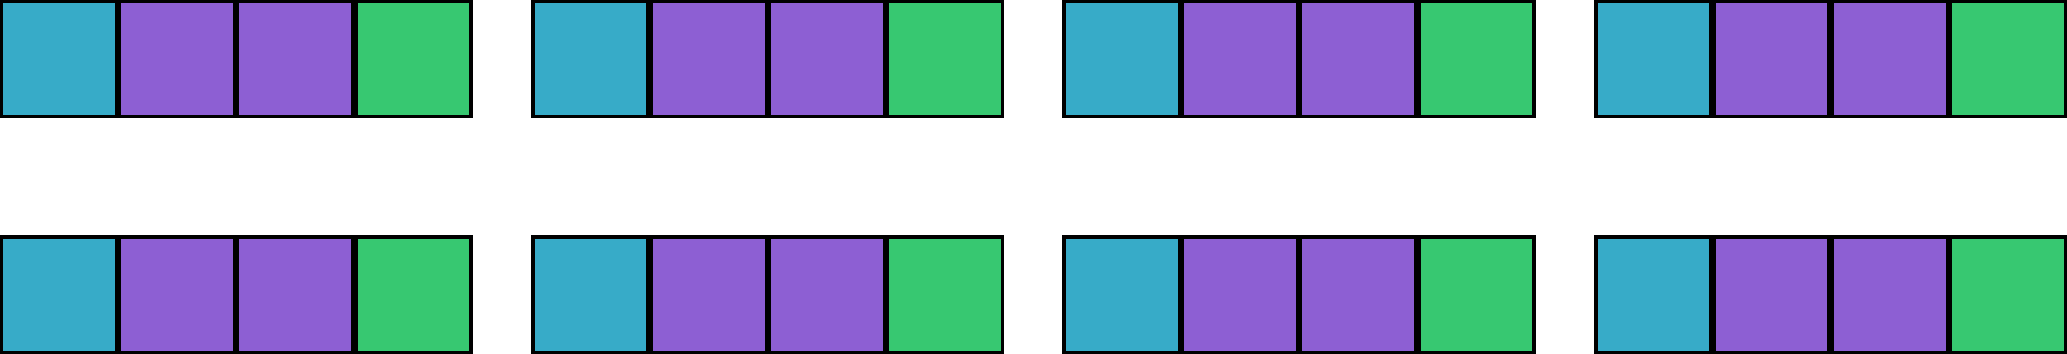
\includegraphics[width=\linewidth]{p1.pdf}
        \caption{1D array of length 8 of a derived type containing a scalar, 2 element array, and scalar. The array is contiguous.}
        \label{sf:synergya}
    \end{subfigure}

    \begin{subfigure}[t]{\linewidth}
        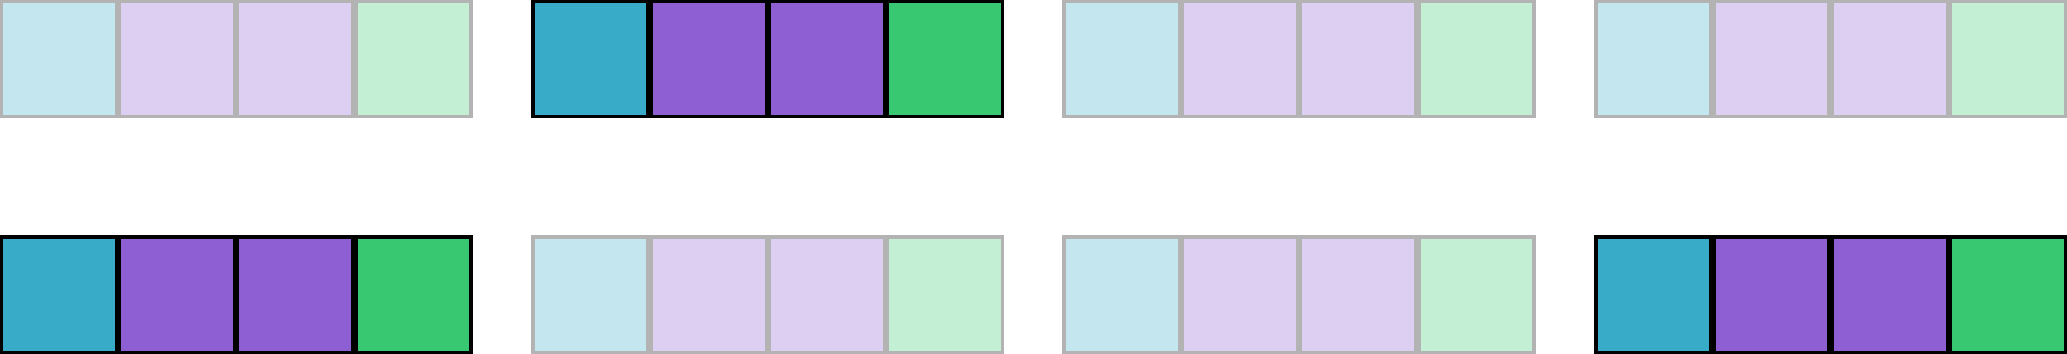
\includegraphics[width=\linewidth]{p2.pdf}
        \caption{Section the array to include only every 2\textsuperscript{nd} item (stride of two) starting from the 2\textsuperscript{nd} element. The array is no longer contiguous.}
        \label{sf:synergyb}
    \end{subfigure}

    \begin{subfigure}[t]{\linewidth}
        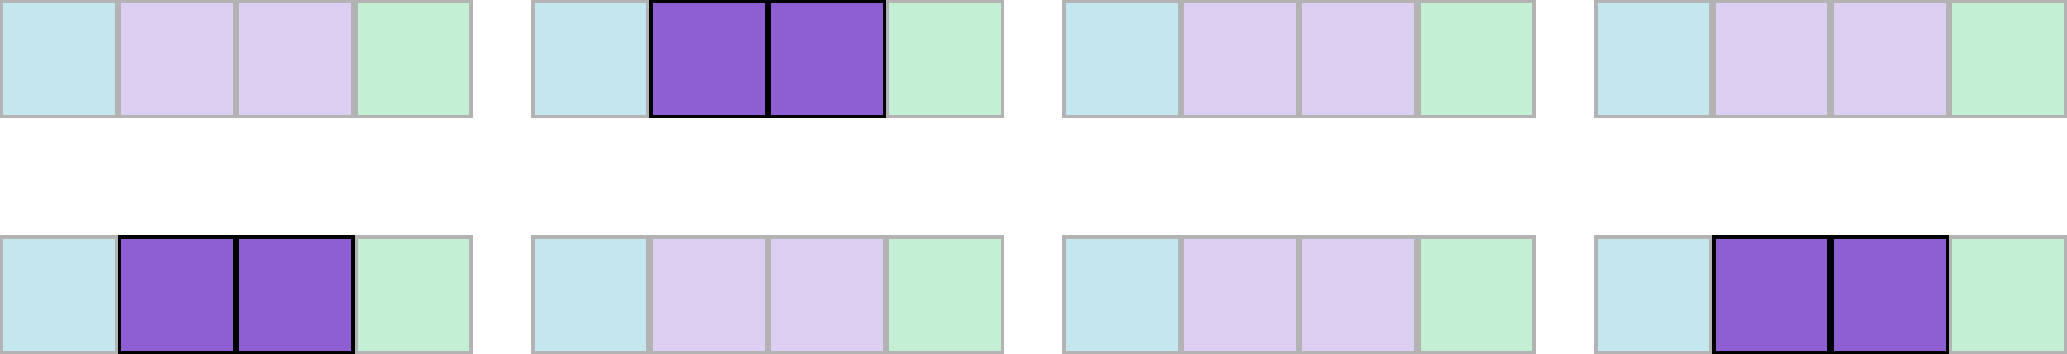
\includegraphics[width=\linewidth]{p3.pdf}
        \caption{Select only the arrays within each element of the array section found in \cref{sf:synergyb}.}
        \label{sf:synergyc}
    \end{subfigure}

    \begin{subfigure}[t]{\linewidth}
        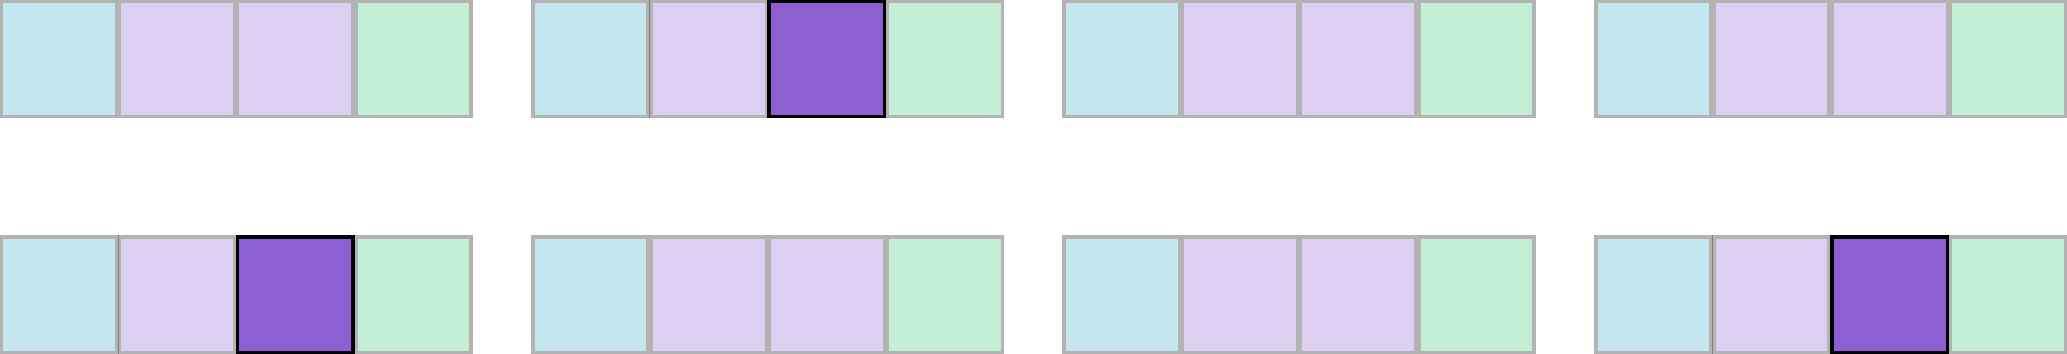
\includegraphics[width=\linewidth]{p4.pdf}
        \caption{Section the array to only select the second item of the array of arrays in \cref{sf:synergyc}.}
        \label{sf:synergyd}
    \end{subfigure}
    \caption{The order can be different, but all these changes must somehow be accounted for within the C descriptor.}
    \label{f:synergy}
\end{figure}

It is important to note that the C descriptor functions do no data copying as that would severely impact performance. Instead, what they do is update the information in the C descriptor such that the programme may find the relevant C addresses via pointer arithmetic.

\section{Results and conclusions}

The standard C descriptors and associated functions were successfully implemented and fully tested. They passed all the tests during development. They fail to build with \texttt{clang} because they utilise a \texttt{GCC} expansion that allows one to define structures with variable length arrays (arrays with no explicit length within structures). However, this is being solved by the Sourcery Institute \cite{sourcery} and is merely a case of ``unrolling'' the structure with the variable length array into explicit structures for specific ranks.

The code can be found in the Github repository \newline{}\href{https://github.com/sourceryinstitute/ISO_Fortran_binding}{/sourceryinstitute/ISO\_Fortran\_binding}. The descriptors are now also being implemented by the \texttt{GCC} \texttt{gfortran} developers. They plan on porting the non-standard descriptors and associated programs to use the standard descriptors and functions. They are also being ported into the OpenCoarrays project \cite{ocafp} by the Sourcery Institute.

It is hard to say which future releases will include the full implementation of the C descriptors but the next major \texttt{GCC} release will likely provide partial support\footnote{These features are partially supported by early versions of \texttt{GCC 7} and fully supported by \texttt{GCC 8} and above.}. The OpenCoarrays project is still mostly largely focused on ironing out bugs with platform support and rare edge cases, so it is unlikely the port will be made within the next release. However, support for them might be present in the release of OpenCoarrays 3.0 within the next few years.

\section{Acknowledgements}

I would like to thank Izaak ``Zaak'' Beekman, Soren Rasmusen, Jerry Delisle, Paul Thomas and last but certainly not least Damian Rouson for the opportunity and priviledge to work with them. I have been a fan of the Sourcery Institute since my early days as an undergrad. It was a wonderful and fun time full of learning and merriment. Hopefully my work will contribute to the success and popularity of open-source scientific software.